\documentclass[border=10pt]{standalone}

\usepackage{tikz}
\usepackage{tikzsymbols}
\usetikzlibrary{calc,patterns,shapes.geometric}

\def\centerarc[#1](#2)(#3:#4:#5){\draw[#1] ($(#2)+({#5*cos(#3)},{#5*sin(#3)})$) arc (#3:#4:#5);}

\begin{document}
	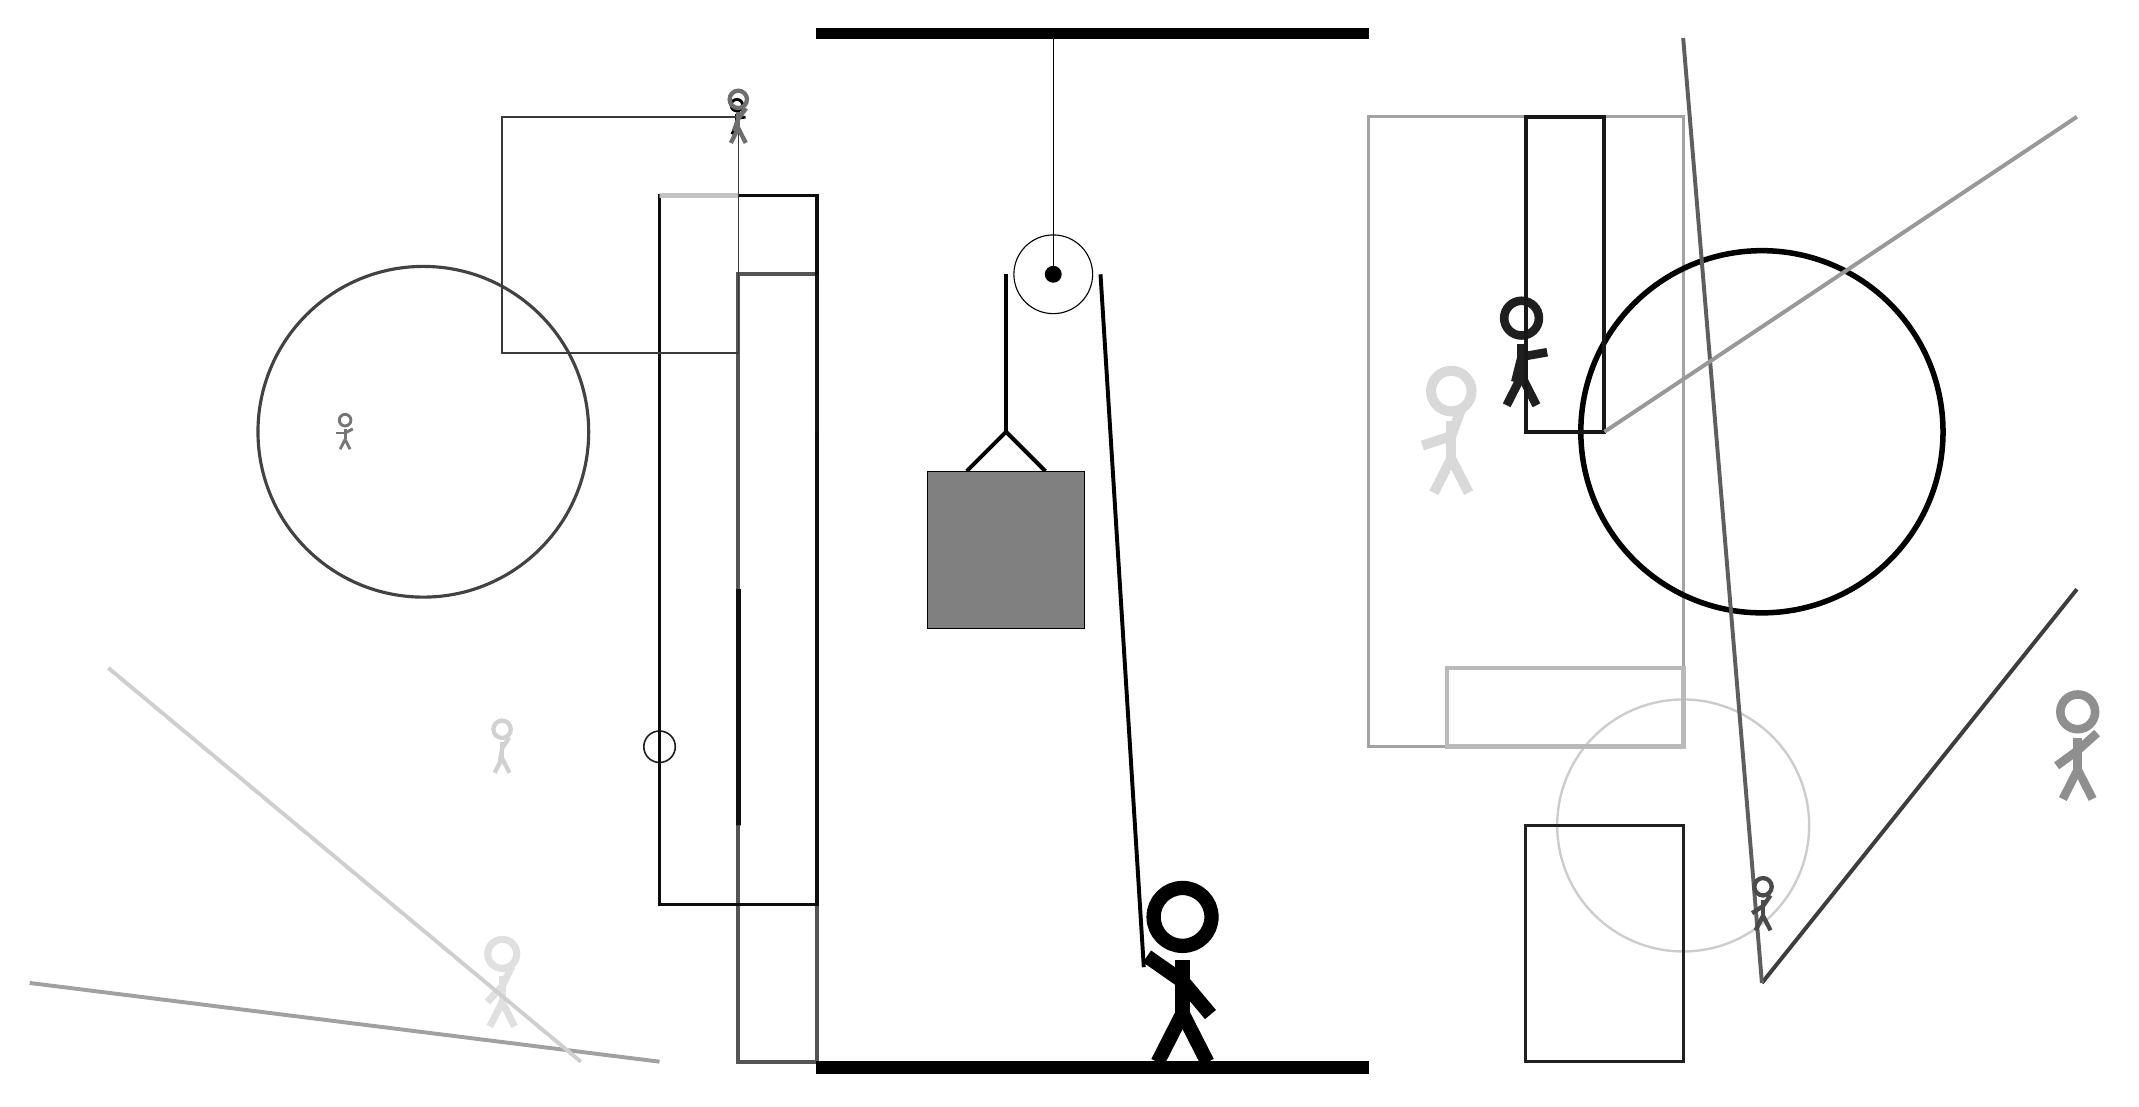
\begin{tikzpicture}
		%%%%% START %%%%%
		
		\draw[fill=black] (-2, 10) rectangle (5, 10.125);
		
		\draw (1, 7) circle (0.5);
		\draw[fill=black] (1, 7) circle (0.1);
		\draw (1, 10) -- (1, 7);
		
		\draw[line width=0.5mm] (-0.1, 4.5) -- (0.4, 5.0) -- (0.9, 4.5);
		\draw[fill=black!50] (-0.6, 4.5) rectangle (1.4, 2.5);
		
		\draw[line width=0.5mm] (0.4, 7) -- (0.4, 5.0);
		\centerarc[line width=0.5mm](1, 7)(0:180:0.6);
		\draw[line width=0.5mm](1.6, 7) -- (2.15, -1.8);
		
		\draw[line width=0.4mm, color=black!36] (5, 9) rectangle (9, 1);
		
		\draw[line width=0.5mm, color=black!76](10, -2) -- (14, 3);
		\draw[line width=0.2mm, color=black!43] (-2, 8) rectangle (-3, 7);
		\draw [line width=0.7mm, color=black!100](10, 5) circle (2.3);
		\node[line width=0.3mm, color=black!18] at (-6, 1) {\Strichmaxerl[3][80][58]};
		\node[line width=0.3mm, color=black!12] at (-6, -2) {\Strichmaxerl[5][47][64]};
		
		\node[line width=0.6mm, color=black!54] at (-8, 5) {\Strichmaxerl[2][0][28]};
		\draw [line width=0.3mm, color=black!20](9, 0) circle (1.6);
		\node[line width=0.5mm, color=black!100] at (-3, 9) {\Strichmaxerl[2][84][6]};
		\draw [line width=0.2mm, color=black!89](-4, 1) circle (0.2);
		
		\draw[line width=0.5mm, color=black!67] (-2, -3) rectangle (-3, 7);
		
		\node[line width=0.7mm, color=black!88] at (7, 6) {\Strichmaxerl[6][76][10]};
		\draw [line width=0.4mm, color=black!74](-7, 5) circle (2.1);
		
		\draw[line width=0.4mm, color=black!95] (-4, -1) rectangle (-2, 8);
		\draw[line width=0.5mm, color=black!37](-4, -3) -- (-12, -2);
		\draw[line width=0.5mm, color=black!63](9, 10) -- (10, -2);
		\draw[line width=0.6mm, color=black!92] (-2, 5) rectangle (-2, 7);
		\draw[line width=0.6mm, color=black!27] (6, 2) rectangle (9, 1);
		\draw[line width=0.4mm, color=black!87] (7, 0) rectangle (9, -3);
		
		\draw[line width=0.5mm, color=black!91] (7, 9) rectangle (8, 5);
		\draw[line width=0.5mm, color=black!40](8, 5) -- (14, 9);
		\draw[line width=0.7mm, color=black!24] (-4, 8) rectangle (-3, 8);
		\draw[line width=0.5mm, color=black!19](-5, -3) -- (-11, 2);
		\node[line width=0.7mm, color=black!44] at (14, 1) {\Strichmaxerl[6][36][42]};
		\draw[line width=0.2mm, color=black!77] (-3, 9) rectangle (-6, 6);
		
		\draw[line width=0.2mm, color=black!76] (7, 8) rectangle (7, 8);
		\node[line width=0.7mm, color=black!71] at (10, -1) {\Strichmaxerl[3][33][55]};
		\draw[line width=0.7mm, color=black!94] (-3, 0) rectangle (-3, 3);
		\node[line width=0.6mm, color=black!57] at (-3, 9) {\Strichmaxerl[3][70][53]};
		\node[line width=0.2mm, color=black!15] at (6, 5) {\Strichmaxerl[7][18][70]};
		\draw [line width=0.7mm, color=black!11](-6, 1) circle (0.0);
		
		\node at (2.6, -1.9) {\Strichmaxerl[10][-35][-50]};
		
		\draw[fill=black] (-2, -3) rectangle (5, -3.15);
		
		%%%%% END %%%%%
	\end{tikzpicture}
\end{document}